% This is a basic Math Paper

\documentclass[12pt]{article}

% Preamble

\usepackage[margin=1in]{geometry}
\usepackage{amsfonts, amsmath, amssymb}
\usepackage{fancyhdr, float, graphicx}
\usepackage[utf8]{inputenc} % Required for inputting international characters
\usepackage[T1]{fontenc} % Output font encoding for international characters
\usepackage{fouriernc} % Use the New Century Schoolbook font
\usepackage[nottoc, notlot, notlof]{tocbibind}
\usepackage{url}
\usepackage{placeins}
\usepackage{multirow}
% Header and Footer
\pagestyle{fancy}
\fancyhead{}
\fancyfoot{}
\fancyhead[L]{\textit{\Large{Experiment 6}}}
\fancyhead[R]{\textit{something}}
\fancyfoot[C]{\thepage}
\renewcommand{\footrulewidth}{1pt}



% Other Doc Editing
\parindent 0ex
\renewcommand{\baselinestretch}{1.2}

\begin{document}
	
	\begin{titlepage} 
		\centering 
		
		%---------------------------NAMES-------------------------------
		
		\huge\textsc{
			MIT World Peace University
		}\\
	
		\vspace{0.75\baselineskip} % space after Uni Name
		
		\LARGE{
			Physics\\
			First Year B. Tech, Trimester 3\\
			Academic Year 2021-22
		}
		
		\vfill % space after Sub Name
		
		%--------------------------TITLE-------------------------------
		
		\rule{\textwidth}{1.6pt}\vspace*{-\baselineskip}\vspace*{2pt}
		\rule{\textwidth}{0.6pt}
		\vspace{0.75\baselineskip} % Whitespace above the title
		
		
		
		\huge{\textsc{
				Measurement of the Energy Band Gap of a Semiconductor
			}} \\
		
		
		
		\vspace{0.5\baselineskip} % Whitespace below the title
		\rule{\textwidth}{0.6pt}\vspace*{-\baselineskip}\vspace*{2.8pt}
		\rule{\textwidth}{1.6pt}
		
		\vspace{1\baselineskip} % Whitespace after the title block

		%--------------------------SUBTITLE --------------------------	
			
		\LARGE\textsc{
			Experiment No. 6
		} % Subtitle or further description
		\vfill
		
		%--------------------------AUTHOR-------------------------------
		
		Prepared By
		\vspace{0.5\baselineskip} % Whitespace before the editors
		
		\Large{
			109054. Krishnaraj Thadesar
			
			Division 9 Batch I3
		}
		
		
		\vspace{0.5\baselineskip} % Whitespace below the editor list
		\today

	\end{titlepage}

	\begin{center}
	{\Large Pledge}\\
	\vspace{0.5cm}
	I solemnly affirm that I am presenting this journal based on my own experimental work. I have neither copied the observations, calculations, graphs and results from others nor given it to others for copying.\\
		\end{center}
	
	\vspace{0.5cm}
	
    \begin{flushright}
	{\large Signature of the student}\\
	\vspace{1cm}
	 \end{flushright}
	
	\section{Aim}
	\noindent
	To measure energy gap of given semiconductor

	
\section{Apparatus}


		\begin{enumerate}
			\item Semiconductor (thermistor with NTC)
			\item Heating arrangement with mini-oven filled with sand powder and
			secondary windings of a step down transfer for controlled electrical
			heating,
			\item Digital Multimeter (DMM) (Refer Fig 7.2)
		\end{enumerate}

\section{Significance of the Experiment}
	\textit{The energy gap, i.e. the gap between valance band and
	conduction band decides the conductivity of a material. The typical energy gaps of the
	semiconductors which are in the range 1 eV to 3 eV impart many useful properties to the
	semiconductors. The ability of the semiconductors to conduct due to electrons as well as holes,
	their ability to convert light in to electricity and electricity in to light, decrease in the resistance
	with temperature are all due to their typical energy gaps. The electronics (PN junction diode,
	NPN or PNP transistor), photonics (LED, laser diode, photodiode, solar cell, LDR etc.) and
	thermistors, are all based on the typical energy gaps of semiconductors. The energy gap of
	silicon (1.1 eV) makes it more applicable than germanium (0.72 eV). This experiment
	demonstrates one of the simplest methods of measuring the energy gap of semiconductors.}
	
\section{Theory}
	\begin{figure}[H]
		\centering
		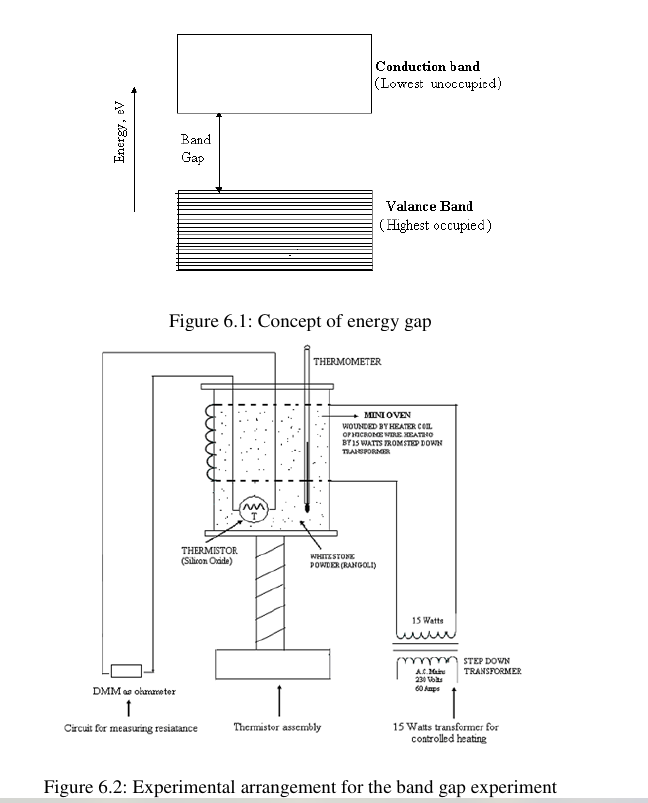
\includegraphics[scale=0.8]{somefig.png}
		\label{it}
	\end{figure}
	Individualatoms are characterized by discrete energy levels. When atoms come together
	and form bonds, their energy levels split and become bands. This happens due to the overlapping
	of electron wave-functions and Pauli’s exclusion principle. Crystalline solids are characterized
	by energy band diagrams. The energy band diagram of a solid is characteristic to it’s atom and
	inter-atomic spacing. The highest occupied band in such energy bands is called as valance band
	while the lowest unoccupied band is called as conduction band. The valance band and
	conduction band are separated by a group of quantum mechanically forbidden energy levels
	called as energy gap (refer Fig 7.1). The size or value of this energy gap varies with the material.
	In conductors like copper, aluminum, gold, silver etc. the energy gap is zero, while it is high in
	insulators like diamond (5 to 6 eV). Elemental semiconductors such as silicon, germanium and
	compound semiconductors such as gallium arsenide, zinc sulphide, gallium phospide, etc are
characterized by intermediate energy gaps (0.66 to 3.6 eV).
The resistance (RT) of a semiconductor having energy gap (Eg) decreases with the
temperature (T), according to following relation

$$
R_{T}=R_{T O} e^{\frac{E_{g}}{2 K T}}
$$
Where $\mathrm{K}$ is the Boltzmann's constant
By taking logarithms and rearranging
$$
\ln R_{T}=\ln R_{T O}+\left(\frac{E_{g}}{2 K}\right) \times \frac{1}{T}
$$
Eqn (7.2) signifies a straight line $(\Rightarrow y=m x+c)$ Thus the graph of $\ln R_{T} V s \frac{1}{T}$ is a straight line having slope $m=\frac{E_{g}}{2 K}$. Thus
$$
E_{g}=2 \mathrm{Km}
$$
Eqn (6.3) provides a simple and straightforward method of measuring energy gap of a semiconductor.



\section{Procedure}
\begin{enumerate}
	 
	\item Connect the circuit as shown in the circuit diagram and get it checked. Connect the terminals of the thermistor to the DMM. Operate DMM in resistance mode and with appropriate scale.
	\item Record the room temperature and corresponding resistance $\left(R_{T}\right)$ of thermistor. Express resistance in $\Omega$ (not in $\mathrm{k} \Omega$ or $\mathrm{M} \Omega$ ).
	\item Start heating the oven by making $\mathrm{AC}$ mains $\mathrm{ON}$. Record decreasing values of resistances (in $\Omega$ ) at different temperatures as shown in the observation table.
	\item Calculate various quantities such as $T(=t+273 \mathrm{~K}), \frac{1}{T}$ and $\ln R_{T}$
	\item Plot the graph of $R_{T} V s T$. This graph exhibits the NTC (Negative Temperature Coefficient) property of thermistor
	\item Plot the graph of $\ln R_{T} V s \frac{1}{T}$. Calculate its slope $(m)$ and the energy gap using Eqn (7.3)
\end{enumerate}

\section{Observations}

\begin{figure}[H]
	\centering
	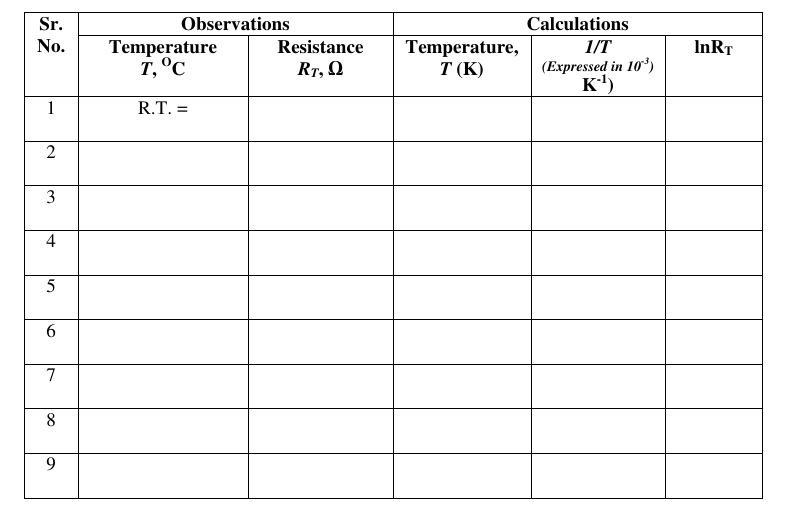
\includegraphics[scale=0.7]{table.png}
	\label{it}
\end{figure}

\section{Calculations}
Slope of the graph of $\ln R_{T} V s \frac{1}{T}=m=$ $\mathrm{K}$
Energy gap, $\quad E_{g}=2 \mathrm{Km}$, where $K=$ Boltzman's constant $=1.37 \times 10^{-23} \mathrm{~J} / \mathrm{K}$
$$
\begin{aligned}
&=2 \times 1.37 \times 10^{-23}\left(\frac{J}{K}\right) \times m(K)=2 \times 1.37 \times 10^{-23}\left(\frac{J}{K}\right) \times \ldots \ldots \ldots(K) \\
&=\ldots \ldots \ldots \ldots \ldots \ldots \ldots . \mathrm{J}=\frac{. \ldots \ldots \ldots \ldots \ldots \ldots \ldots \ldots \ldots(J)}{1.6 \times 10^{-19} \frac{J}{e V}}=\ldots \ldots \ldots \mathrm{eV}
\end{aligned}
$$
Result: The energy gap of given semiconductor (thermistor) is $\mathrm{eV}$
	
\section{Graphs}
\subsection{Plot between Temperature in Kelvin and Resistance in Ohm}
\begin{figure}[H]
	\centering
	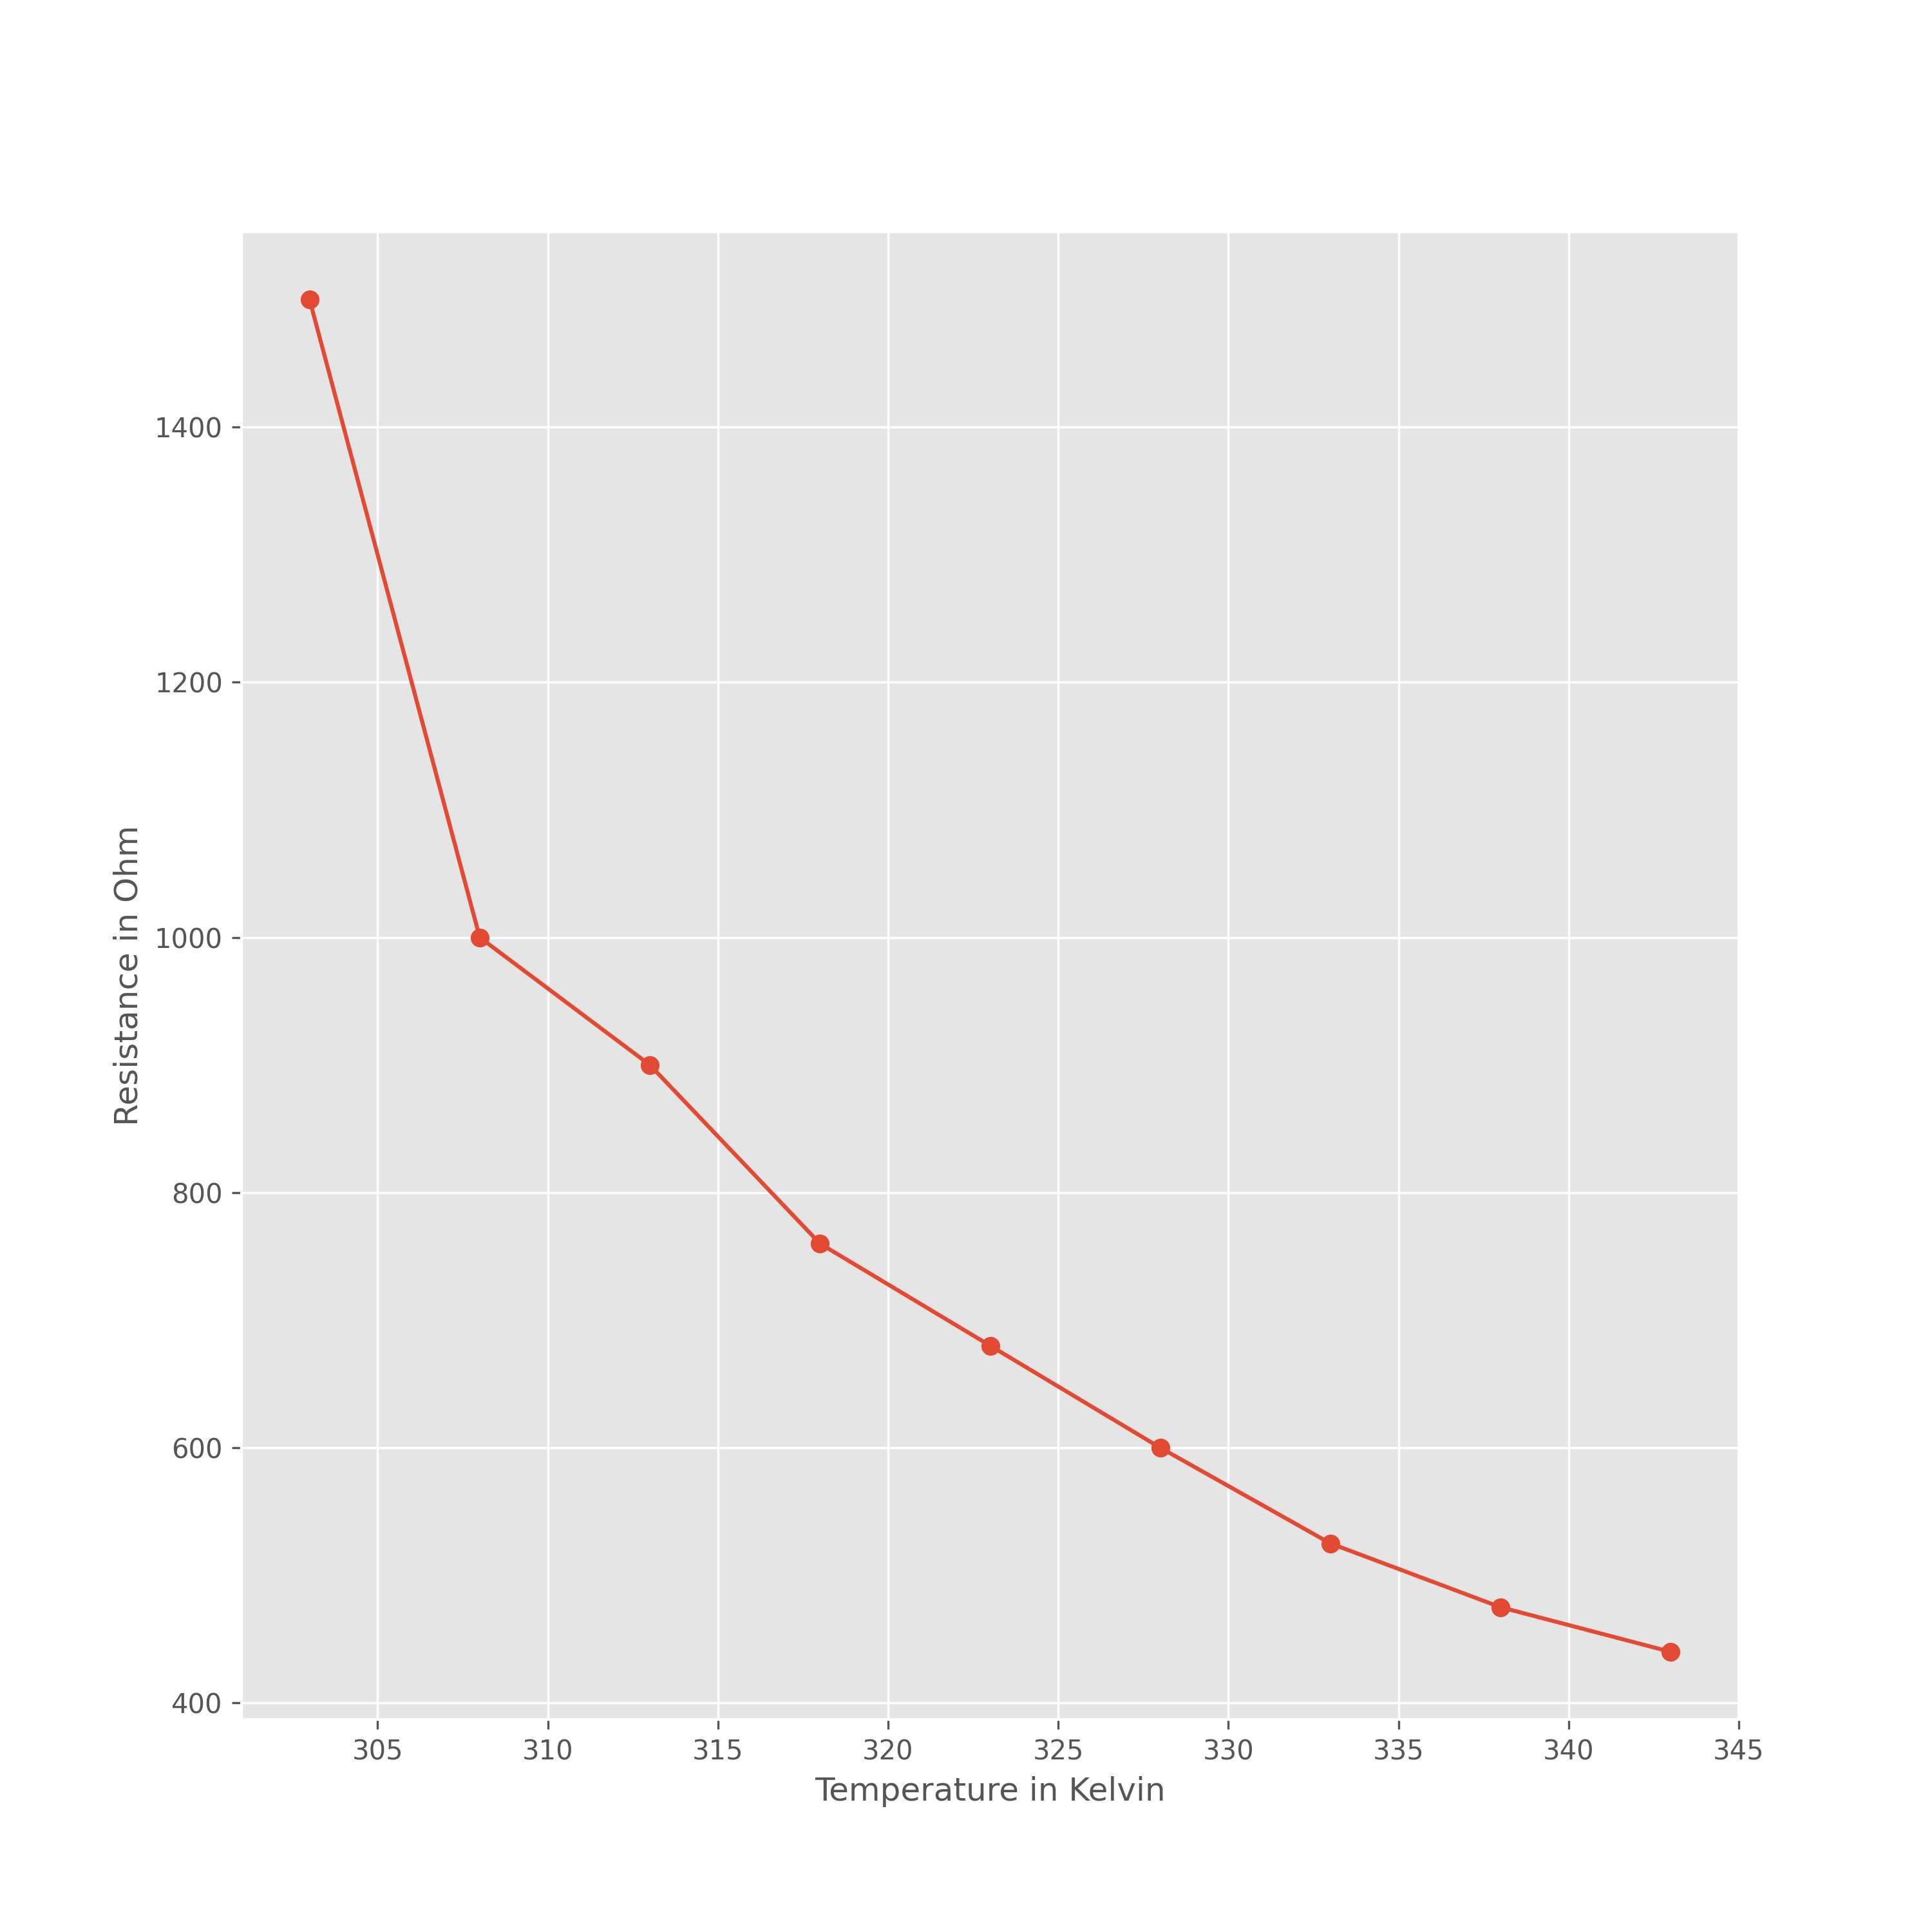
\includegraphics[scale=0.6]{fig.png}
	\label{it}
\end{figure}

\subsection{Plot between $1/Temperature$ in kelvin vs $ln(Resistance)$ in Ohm}
\begin{figure}[H]
	\centering
	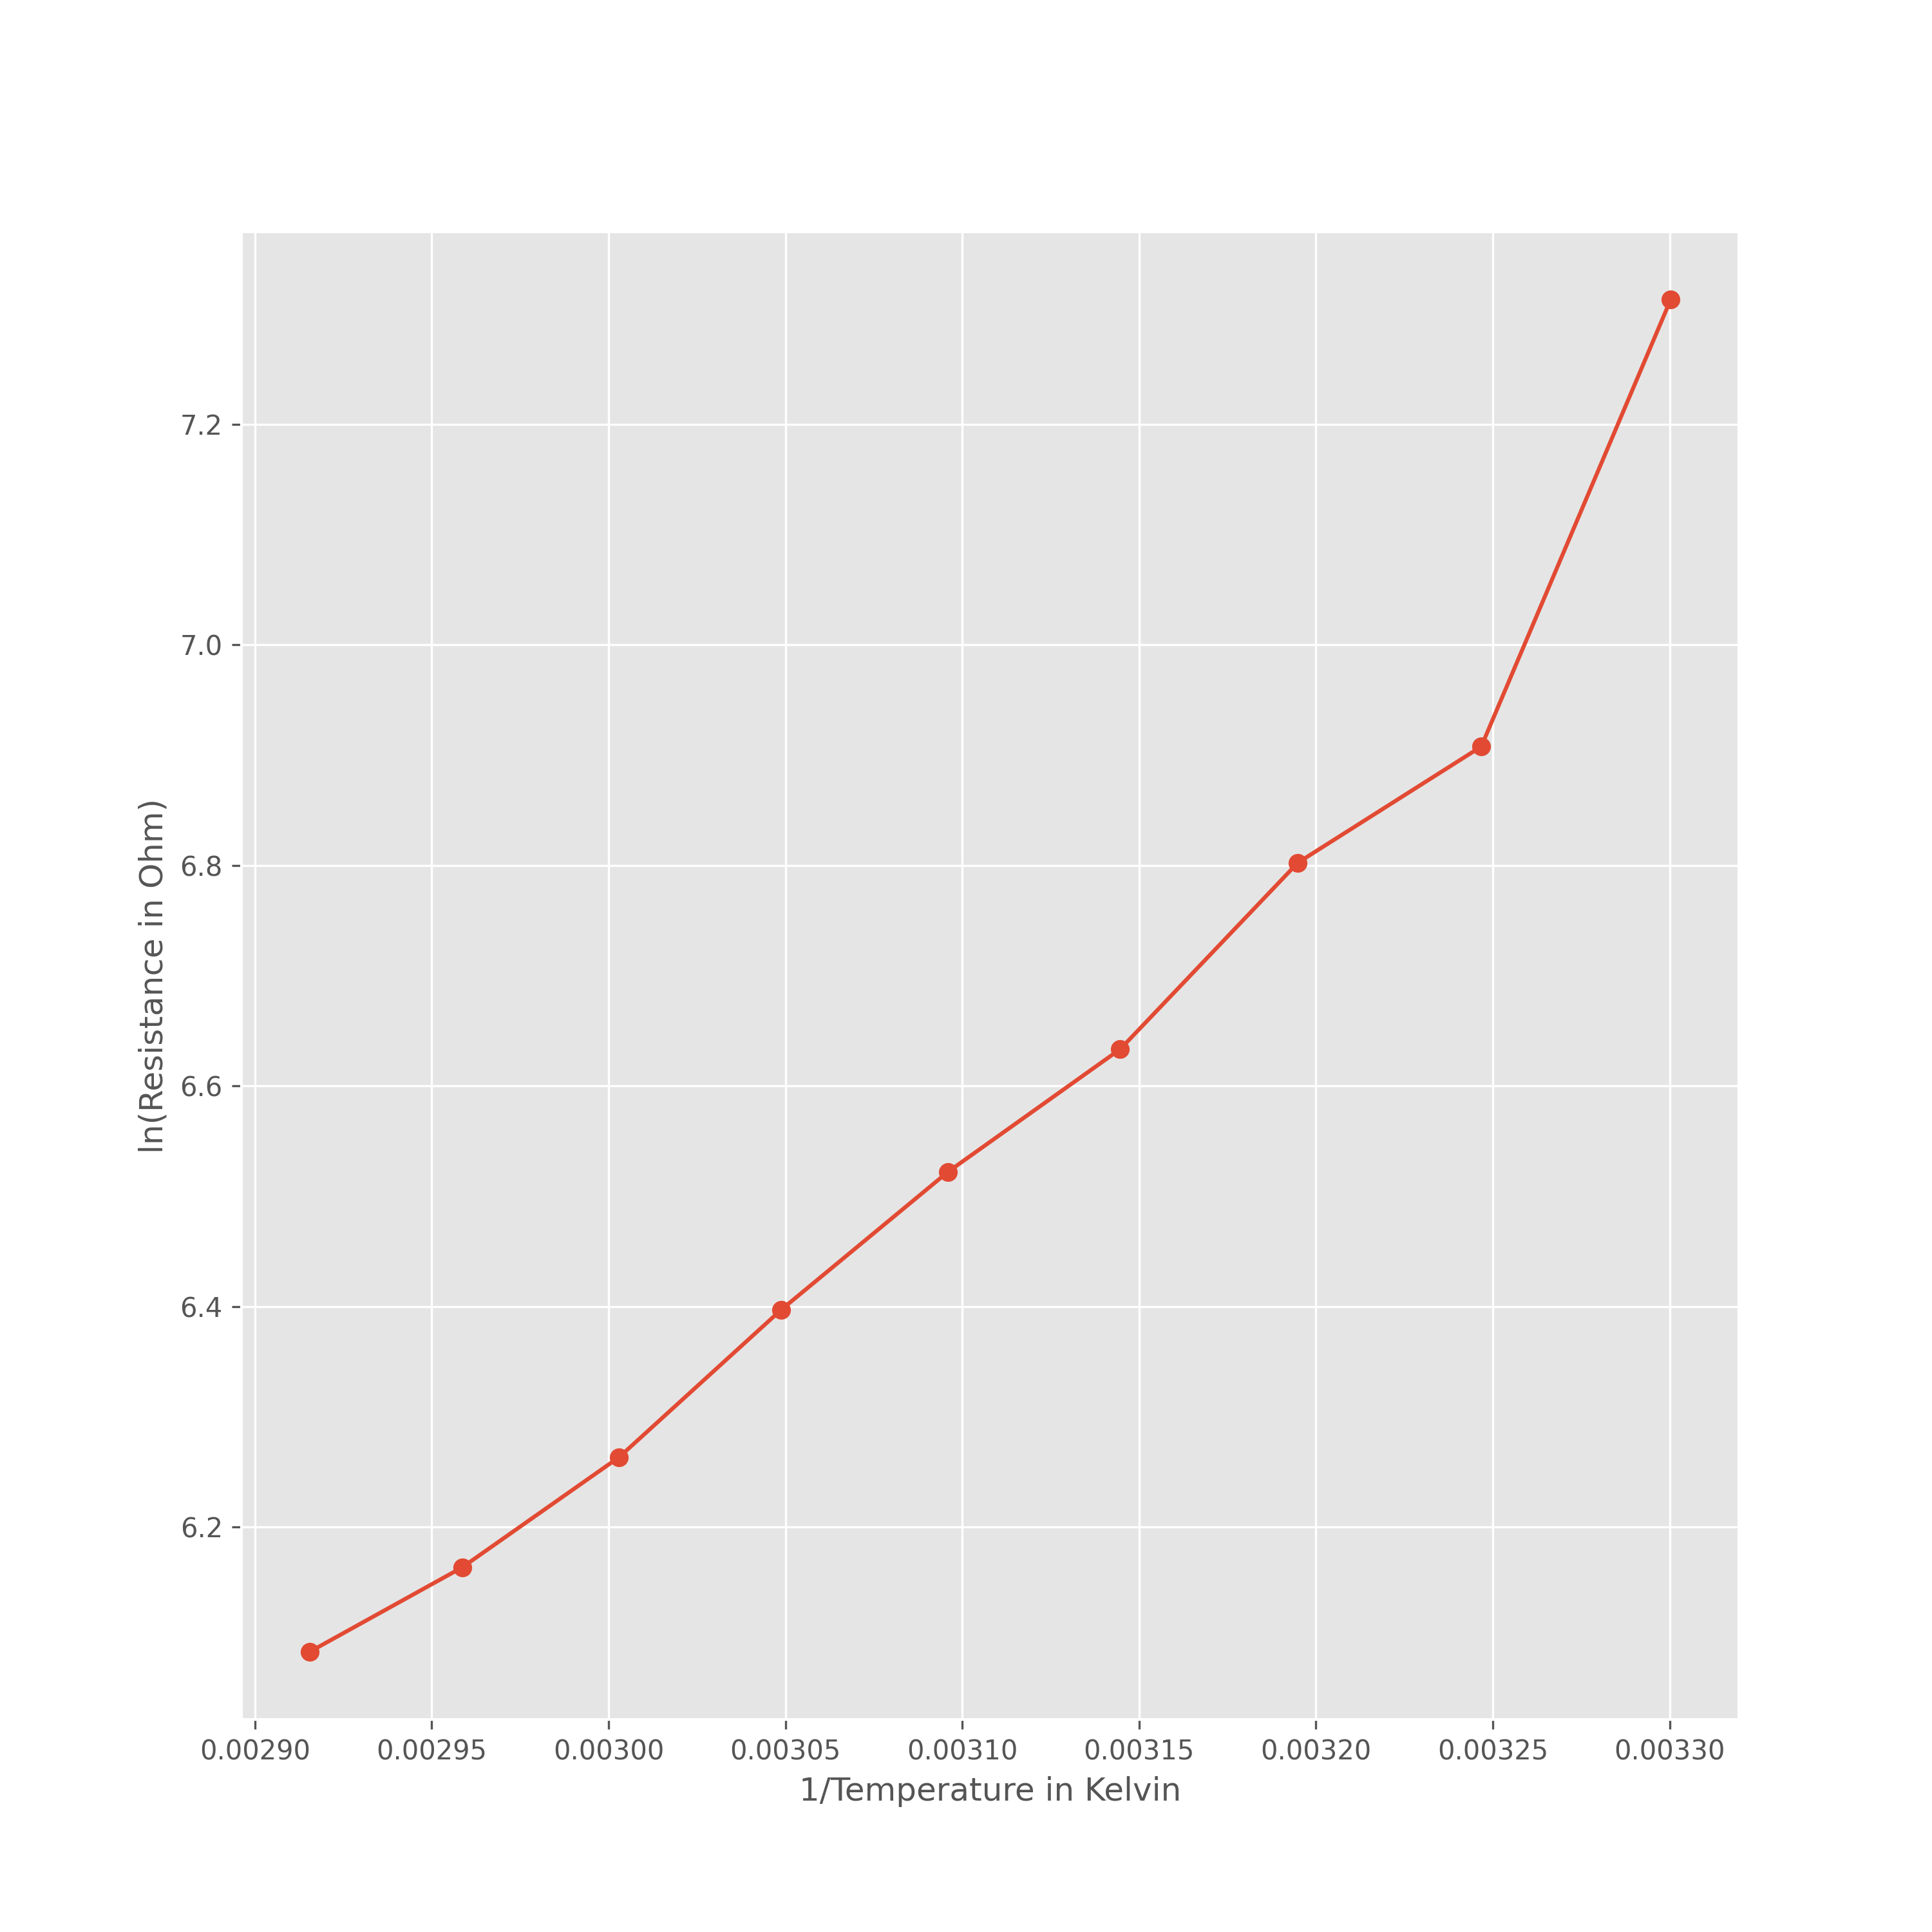
\includegraphics[scale=0.55]{fig2.png}
	\label{it}
\end{figure}

\section{My Understanding of the Experiment}
Semiconductors are special in that their resistance decreases upon increase in temperature due to higher number of electrons being present in the conduction band. 
The rise in temperature basically provides thermal energy to those electrons, so that they can jump across the forbidden band gap, and go to the conduction band. So naturally
for every substance, having its own unique band gap, the temperature required to bring them to the conduction band is also unique. So there exists a relation between the 
band gap, and the temperature. It is using this relation, and property that the energy band gap of a semiconductor can be calculated, and different semiconductors can be recognized based
on it. 
\end{document}